% Supplement: tracker integration, acquisition clocks, controls, and retained evidence.
\documentclass[conference,letterpaper,10pt]{IEEEtran}
\usepackage{amsmath,amssymb,bm,booktabs,array,graphicx,cite,balance}
\usepackage[hidelinks]{hyperref}
\hypersetup{pdftitle={Polynomial Nuisance Profiling: Supplementary Material},pdfauthor={Anonymous Authors}}
\graphicspath{{recovery_bootstrap_figures/}}
\newcommand{\sk}[1]{[#1]_\times}
\renewcommand{\thesection}{S-\Roman{section}}
\renewcommand{\thetable}{S-\Roman{table}}
\renewcommand{\thefigure}{S-\arabic{figure}}
\renewcommand{\theequation}{S-\arabic{equation}}
\title{Polynomial Nuisance Profiling for Range--Inertial Initialization\\Supplementary Material}
\author{\IEEEauthorblockN{Anonymous Authors}}
\begin{document}
\maketitle

\section{Tracker Integration and Time Origins}
This material records the common integration policy and retained controls. It does not expand the initialization paper's contribution to complete-filter convergence. The original Oursland--Mehrabian setting uses TDoA and a tag lever arm\cite{oursland2024}; these TWR, zero-lever-arm experiments do not directly rank that original system.

\subsection{Three Time Coordinates}
The loader first subtracts the existing $0.20$ s correction from IMU and TWR acquisition timestamps and references them to the first valid OptiTrack timestamp. Call this clock $t_L$. Initial gravity alignment and static bias estimation use the approximately 1.5 s prefix. Preparation retains samples with $t_L\ge1.5$ s and resets the clock to the first retained sample, $t_C=t_L-t_{L,0}$. Here $t_{L,0}$ is about 1.50 s (1.51 s in the square log), rather than a searched first-range timestamp.

The first fixed 2 s capture starts at $t_C=0$ and hands off at the first sample with $t_C\ge2$ s. Thus its reported startup unavailability is about 2 s on the post-prefix clock, or about 3.5 s after the loader origin. The shared trajectory-RMSE interval $t_C\ge8.1$ s begins about 9.6 s after that origin. Window-study requests at 5, 10, 20, and 30 s use $t_C$ and the last arrived cached sample no later than the request; truth is interpolated at that actual endpoint.

The scripted outage removes transactions on $t_C\in[15,25)$ s. The estimator is not told the end time: recapture starts when a new changed positive range follows an observed inter-arrival gap greater than 1 s. The existing tracker's propagated output remains visible during the capture window, and its error remains in the score.

\subsection{State and Covariance Handoff}
The same tracker uses error ordering $[\theta,v,p,b_g,b_a]$. For physical errors consisting of body-right attitude and additive world velocity/position, the map to the right-invariant chart is
\begin{equation}
 C_X=\begin{bmatrix}
 R&0&0&0&0\\
 \sk{v}R&I&0&0&0\\
 \sk{p}R&0&I&0&0\\
 0&0&0&I&0\\0&0&0&0&I
 \end{bmatrix},\qquad P_r=C_XP_eC_X^\top .
\end{equation}
The endpoint yaw increment maps to $R^\top e_3$ in body attitude coordinates. Position--velocity--yaw cross terms are retained, with broad priors for unobserved directions and empirical standard-deviation floors of 0.15 m, 0.20 m/s, and 0.10 rad. This regularized IRLS curvature is not a calibrated posterior. A singular-information pseudoinverse alone would incorrectly assign zero variance to its nullspace.

With left group injection, corresponding to $X_{\rm true}\hat X^{-1}$, the range Jacobian is
\begin{equation}
 H_r=\begin{bmatrix}-n^\top\sk{p}&0&n^\top&0&0\end{bmatrix}.
\end{equation}
Chart conversion and reset are applied at the current state. Range updates use a normalized innovation gate of 12.25 and Huber threshold 2 immediately after the new window handoff. Capture measurements are consumed once: only subsequent events enter the initialized tracker. Integration and calibration correlations are not fully propagated by this prototype.

An adaptive control tries 2, 4, and 8 s windows and accepts when fixed-bias projected yaw information is at least $1/(0.35\,{\rm rad})^2$ and normalized residual RMS is at most 3. Fixed 2 s CV, Local, Uniform-12, and Profile-1 windows hand off after fitting without this adaptive acceptance test. These are engineering thresholds; the paper's uncertain-bias ambiguity explains why they do not certify heading.

\section{Retained Complete-Filter Results}
Eight policies on six evaluation logs with and without the outage give 96 existing replays. Stable success requires position error $\le0.5$ m for the complete remaining log with at least 5 s after the last threshold crossing. The square log fails this sustained condition for the fixed-window methods despite a terminal five-second RMSE of about 0.39 m. Finite large errors and missing output are retained.

\begin{table*}[t]
\caption{Existing full replays, six logs per regime. RMSE is the median across logs on $t_C\ge8.1$ s. Maximum is across all available samples and all six logs, including propagated outage/recapture outputs. Startup is on $t_C$; it excludes the static prefix. Values are metres unless specified.}
\centering
\setlength{\tabcolsep}{5pt}
\begin{tabular}{lrrrrrrr}
\toprule
&\multicolumn{4}{c}{Continuous ranging}&\multicolumn{3}{c}{Ten-second outage}\\
\cmidrule(lr){2-5}\cmidrule(lr){6-8}
Method&Success&RMSE&Max.&Startup (s)&Success&RMSE&Max.\\
\midrule
Centroid InEKF&4/6&0.302&$2.08\times10^4$&0&4/6&7.923&$2.08\times10^4$\\
Lifted capture&5/6&0.285&16.27&0&5/6&1.387&17.65\\
Lifted, gate from start&4/6&0.285&$2.18\times10^3$&0&4/6&1.815&$6.12\times10^3$\\
Robust CV window&5/6&0.285&1.504&2&5/6&2.349&25.86\\
Local inertial window&5/6&0.285&1.504&2&5/6&2.164&27.72\\
Uniform-12 inertial&5/6&0.285&1.504&2&5/6&2.164&27.72\\
Profile-1 inertial&5/6&0.285&1.504&2&5/6&2.164&27.72\\
Adaptive profile&4/6&0.283$^\dagger$&1.536&4$^\ddagger$&5/6&2.249$^\dagger$&22.62\\
\bottomrule
\end{tabular}
\par\vspace{3pt}\footnotesize
$^\dagger$Adaptive common-interval availability is 83.3\% with continuous ranging and 94.4\% with an outage; conditional RMSE is not comparable to a fully available output.
$^\ddagger$Median startup; one continuous-ranging log never initializes. All other policies have 100\% common-interval availability. Historical lifted controls publish during acquisition and use their own covariance/warm-up policy, so maximum errors combine accuracy and availability differences.
\end{table*}

Historical lifted capture disables hard rejection and Huber weighting for the first 256 valid updates. A separate truth-initialized first-second diagnostic isolates this policy interaction; it is not a cold-start result. In the random log, a corrected-range error of 7.883 m produces a 34.117 m position jump with only 0.0091 rad attitude injection. Immediate hard gating limits the diagnostic peak to 0.324 m, but a narrow prior around a displaced state can conversely reject the ranges needed for acquisition. These controls motivate a separate acquisition policy without proving one universal gate.

A ten-variable $p_T,v_T,\psi,\delta b_a$ extension uses the reanchored double integral of $Q$, a $0.10\,{\rm m/s^2}$ Gaussian bias prior, and the same tracker. Its data-only yaw information excludes the prior. Sixty existing replays do not show improved full-system recovery. For 2/4/8 s windows, median common-interval RMSEs are $0.285/0.284/0.289$ m normally and $2.332/4.349/11.550$ m with the outage; the 8 s version reaches 93.02 m while output propagates during the longer wait. These are retained negative results.


\section{Calibration and Bias Controls}
The physical IMU stress test supplies 200 Hz specific force and angular-rate samples over 4 s, with yaw-free attitude
\begin{equation}
 Q(t)=R_y(8^\circ\sin1.3t)\,R_x(10^\circ\sin0.9t).
\end{equation}
Specific force is $Q_k^\top(a_k-g)$ and gyro increments use $\log(Q_k^\top Q_{k+1})^\vee/0.005$. Truth and estimator share held-sample propagation and endpoint reanchoring. Ideal, mild, and moderate levels have independent component standard deviations $(\sigma_a,\sigma_g,\sigma_{\rm tilt})=(0,0,0)$, $(0.02,0.002,0.5^\circ)$, and $(0.10,0.01,2^\circ)$, with acceleration in $\mathrm{m/s^2}$ and gyro rate in rad/s. There is no added IMU white noise; this is combined calibration mismatch.

\begin{table}[t]
\caption{Existing $K=1$ calibration test: 200 paired seeds per level. Misses compare the twelve-start reference using $\max(10^{-3},10^{-5}|J_{12}|)$, unlike the new five-method joint-best comparison. Errors are position/physical-heading 95th percentiles (m/$^\circ$).}
\centering
\begin{tabular}{llrr}
\toprule
Level&Method&Misses&Position / heading\\
\midrule
Ideal&Local&53&4.221 / 161.26\\
&Profile-1&0&0.546 / 3.58\\
&Uniform-12&0&0.546 / 3.58\\
Mild&Local&57&4.254 / 161.05\\
&Profile-1&0&1.031 / 16.90\\
&Uniform-12&0&1.031 / 16.90\\
Moderate&Local&65&5.902 / 156.75\\
&Profile-1&31&4.698 / 52.10\\
&Uniform-12&0&4.223 / 133.85\\
\bottomrule
\end{tabular}
\end{table}

The controlled constant-world-bias study uses 1,000 paired seeds per motion and bias scale, with scales $0,0.1,0.3\,{\rm m/s^2}$. Under excited motion at scale 0.3, fixed-$K=1$/free-$K=2$ median position errors are $0.737/0.073$ m and heading errors $7.67/0.92^\circ$. That comparison additionally changes outer refinement count (one versus two), so it cannot isolate model order. The matched two-translation-initialization physical-IMU table in the main paper addresses that confound. Under constant acceleration, all free-bias headings are rejected for negligible data information; this is unavailability, not zero heading error.

\begin{figure}[t]
 \centering
 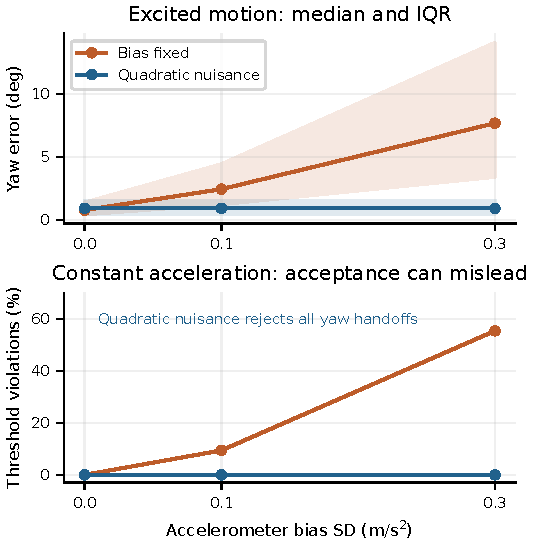
\includegraphics[width=\columnwidth]{bias_tradeoff.pdf}
 \caption{Controlled world-bias study. $K=1$ uses one outer refinement and $K=2$ two, so this figure is not a matched computation ablation. The constant-acceleration diagnostic uses only the information threshold; rejection of every heading means unavailable heading. Excited-motion gains are conditional on this model.}
\end{figure}

\begin{figure*}[t]
 \centering
 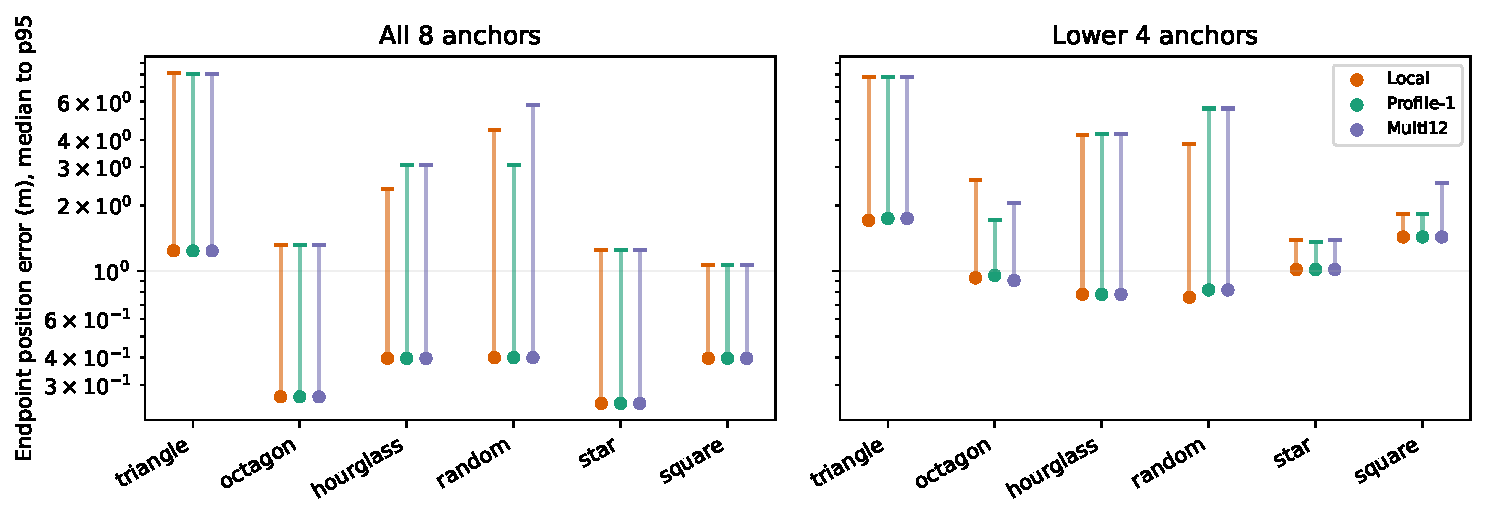
\includegraphics[width=0.96\textwidth]{endpoint_position_by_log.pdf}
 \caption{Real-window endpoint position: median dots and 95th-percentile caps within each recording and anchor layout (44 correlated configurations per policy). These ranges are descriptive error summaries, not uncertainty intervals. Lower residuals do not ensure better physical error.}
\end{figure*}

\section{Window Computation}
For the CV linear translation initialization, let
\begin{align}
 A_i&=[1,\tau_i,\tau_i^2,-a_i^\top,-\tau_i a_i^\top],\\
 b_i&=\tfrac12(r_i^2-\sigma_i^2-\|a_i\|^2),\qquad
 w_i=\frac{1}{\max(r_i\sigma_i,\sigma_i^2)} .
\end{align}
The last six coefficients of the weighted least-squares solution give the first position/velocity seed; the second is the anchor centroid and zero velocity. Each is robustly refined in the CV model and the lower raw cost is retained. Both this linear solve and nuisance projection use a $10^{-10}$ relative singular-value cutoff. These CV weights differ from the inertial lift's variance-based weights given in the main paper. Synthetic uniform yaw seeds are $-\pi+2\pi j/M$, $j=0,\ldots,M-1$; real uniform seeds form the same circular sets.

The main paper's new computation experiment uses the i5-12600KF. Earlier complete studies and the saved real-window sequential timing use the source-study Core Ultra 7 265KF. Function counts describe work; wall times from these hosts must not be pooled. Every evaluation count includes both common CV solves and all yaw refinements. SVD and root enumeration enter elapsed time but not the function-evaluation count.

\begin{table}[t]
\caption{Existing real-window policies: 528 correlated configurations per method. Times are median/95th percentile (ms) on the historical sequential subset (12 configurations, 10 repeats). Endpoint error is the configuration-weighted 95th percentile in metres.}
\centering
\setlength{\tabcolsep}{3.4pt}
\begin{tabular}{lrrrr}
\toprule
Policy&Miss&Total evals&Time (ms)&$p_{95}$\\
\midrule
Local&87&36,157&15.54 / 63.35&4.241\\
Profile-1&40&32,632&13.28 / 65.58&4.084\\
Profile-2&28&47,466&17.79 / 85.83&4.084\\
Profile-all&11&93,690&37.01 / 158.54&4.084\\
Uniform-4&12&85,229&33.44 / 139.58&4.241\\
Uniform-12&0&216,893&83.08 / 364.02&4.241\\
\bottomrule
\end{tabular}
\end{table}

Real windows use the public TU Delft data\cite{pfeifferdata2021}, with six exposed evaluation logs on 2021-02-12, identified by timestamp and motion: 09:43:34 triangle, 09:46:15 octagon, 09:51:57 hourglass, 09:56:09 random, 10:09:28 star, and 13:43:51 square.

\bibliographystyle{IEEEtran}
\bibliography{recovery_bootstrap_refs}
\end{document}
